\section{Background}
\label{sec:cfa:background}

This section begins with some background on video
quality prediction.
 Then, we articulate two key
challenges faced by any video quality prediction system:
(1) The factors affecting video quality are complex, so
we need expressive models; (2) Quality changes
rapidly, so models must be updated in near real-time by
recent quality measurements. We also argue why
existing solutions do not address these challenges.


\subsection{Data-Driven Quality Prediction}
\label{sec:cfa:background:prediction}

Prior work has made the case for a quality optimization 
system (Figure~\ref{fig:globalsystem}) that uses a 
{\em prediction oracle} to suggest the best parameter 
settings (e.g., bitrate, CDN) to optimize quality 
(e.g.,~\cite{sigcomm12,balachandran2013analyzing,
mukerjee2015practical,sigcomm12cdnmulti,c3}).  
Seen in a broader context, this predictive approach 
can be applied beyond Internet video
(e.g.,~\cite{aggarwal2014prometheus,
sambasivan2011diagnosing,
choffnes2010crowdsourcing, velox-cidr,
spand}).

\begin{figure}[t]
\centering
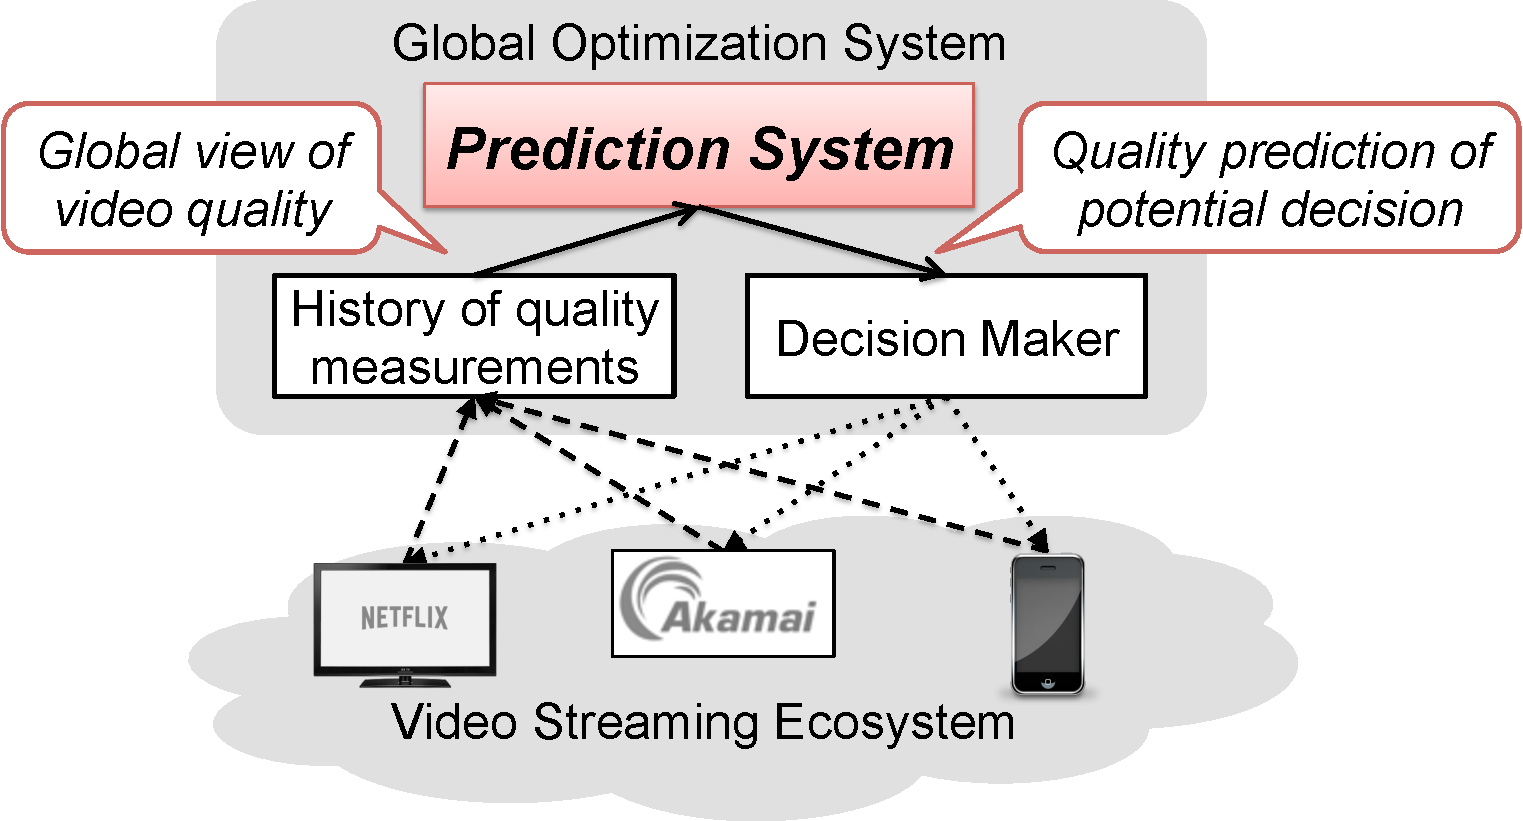
\includegraphics[width=.7\textwidth]{figures/cfa-controlplane-overview.pdf}
\caption{Overview of a \ControlPlane and the crucial role 
of a prediction system.}
\label{fig:globalsystem}
\end{figure}

In the context of video streaming, 
most video service providers today allow a 
video client (player) to switch CDN and bitrate 
among a set of available choices~\cite{sigcomm12,
c3,sigcomm12cdnmulti}.
%Today's video delivery systems allow each video client 
%(player) to switch CDN and bitrate among a set of 
%available choices. 
%\camera{Multi-CDN and multi-bitrate is commonly used by streaming video sites.}
These switches have little overhead and can be
performed at the beginning of and during a video 
playback~\cite{dash}. 
%\myparatight{Need for quality prediction}
Our goal then is to choose the best CDN and 
bitrate for a client by {\em accurately predicting 
the video quality of each hypothetical choice of 
CDN and bitrate}. 
In theory, if we can accurately predict the 
quality of each potential decision, then we 
can identify  the optimal decision.


To this end, we envision a prediction system that 
uses a {\em global view} of quality measurements to 
make predictions for a specific video session. % (i.e., pair of client and decision).
It learns a {\em prediction function} for each 
quality metric
$Pred:2^\HSessionFullSet\times\HSessionFullSet\mapsto \HReal$,
which takes as input a given set of historical 
sessions $\HSessionSet \in 2^\HSessionFullSet$ 
whose quality  is already measured, and a new 
session $\HSession\in\HSessionFullSet$, and 
outputs a quality prediction $p\in\HReal$ for 
$\HSession$.


%\myparatight{Quality metrics and session features} 
Each quality measurement %is a video session viewing a video 
summarizes the quality of a video session
for some duration of time (in our case, one minute). 
It is associated with values of four 
{\em quality metrics} (as defined in 
Section~\ref{subsec:related:video-qoe}) and 
a set of {\em features}
(summarized in Table~\ref{tab:features}).  
By feature,  we refer to the type of attribute 
(e.g., \fCDN), rather than value of these attributes 
(e.g., $\fCDN=Akamai$)
In general, the set of features depends on the degree 
of instrumentation and
what information is visible to a specific provider. 
For instance, a CDN may know the location of servers, 
whereas a third-party optimizer~\cite{conviva} may 
only have information at the CDN granularity. 
Our focus is not to determine the best set of 
features that should be recorded for each session, 
but rather engineer a prediction system that can 
take  an arbitrary set of features as inputs and 
extract the relationships between these features
and video quality. In practice, the above set of 
features can already provide accurate predictions 
that help improve quality.
% , and our approach can naturally include more
% features as they become available. 


\begin{table}[t!]
%\begin{footnotesize}
\begin{tabular}{p{3.8cm}|p{12cm}}
%{\bf Metrics} & {\bf Description} \\ \hline
%BufRatio & Fraction of time a session spends in buffering 
%(smooth playback is interrupted by buffering). \\ \hline
%AvgBitrate & Time-weighted average of bitrates in a session. \\ \hline
%JoinTime & Delay for the video to start playing from the 
%time the user clicks ``play''. \\ \hline
%Video start failure (VSF) & Fraction of sessions that fail to
% start playing (e.g., unavailable content or overloaded 
% server)\tablefootnote{For one session, VSF is zero if it 
% starts successfully, one otherwise.}. \\ \hline
{\bf Features} & {\bf Description} \\ \hline 
 \fASN &  Autonomous System to which client IP belongs. \\ \hline 
 \fCity &  City where the client is located.  \\ \hline
 \fConnectionType &  Type of access network; e.g.,  
 mobile/fixed wireless, DSL, fiber-to-home. \\ \hline
 \fPlayer & e.g.,  Flash, iOS, Silverlight,  HTML5. \\ \hline 
 \fSite & Content provider of requested video contents.\\ \hline%\tablefootnote{We use the terms site and content provider interchangeably.}. \\ \hline
 \fLiveOrVoD & Binary indicator of live vs.\ VoD content.\\ \hline 
 \fContentName & Name of the requested video object.\\ \hline 
 \fCDN &  CDN a  session started with. \\ \hline
 \fBitrate &  Bitrate value the session started at.
\end{tabular}
%\end{footnotesize}
\vspace{-0.2cm}
\caption{Quality metrics and session features associated 
with each session. 
\fCDN and \fBitrate refer to initial CDN/bitrate values as 
we focus on initial selections.}
\label{tab:features}
%\vspace{-0.5cm}
\end{table}

Our dataset consists of 6.6 million quality 
measurements collected from 2 million clients 
using 3 large public CDNs distributed across 
168 countries and 152 ISPs.

Next, we show real examples of the complex factors 
that impact video quality, and the limitations of strawman
solutions in capturing these relationships.

\subsection{Challenge 1: Complex QoE-Determining Factors}
\label{subsec:expressive}

\mypara{
High-dimensional relationship between video quality
and session features} 
Video quality could be impacted by {\em combinations} 
of multiple components in the network. 
Such high-dimensional effects make 
it harder to learn the relationships between video 
quality  and features, in contrast to simpler settings 
where features affect quality independently 
(e.g., assumed by Naive Bayes).
%quality prediction challenging since the 
%relationship between video quality and 
%features is more complex than if the impact of 
%individual features on quality is independent 
%(which is assumed by algorithms like Naive Bayes).




%\noindent\underline{Example of high dimensionality:}
%Here is an illustrative real-world example of high 
%dimensionality. 
In a real-world incident,
video sessions of Comcast users in Baltimore who watched 
videos from Level3 CDN experienced high failure rate (VSF) 
due to congested edge servers, shown by the blue line in 
Figure~\ref{fig:timeseries-expressive-model}.
The figure also shows the VSF of sessions sharing the same
values on one or two features with the affected sessions; 
e.g., all Comcast sessions across different cities and CDNs. 
In the figure, the high VSF of the affected sessions cannot be 
clearly identified if we look at the sessions 
 that match on only one or two features.
%does not suffice to clearly 
%none of the individual features or 
%two-feature combinations can clearly 
%show the high VSF of the affected sessions.
Only when three features of \fCDN (``Level3''), 
\fASN (``Comcast'') and \fCity (``Baltimore'') 
are specified (i.e., blue line), can we detect the 
high VSF and predict the quality of 
affected sessions accurately. 

\begin{figure}[t!]
\centering
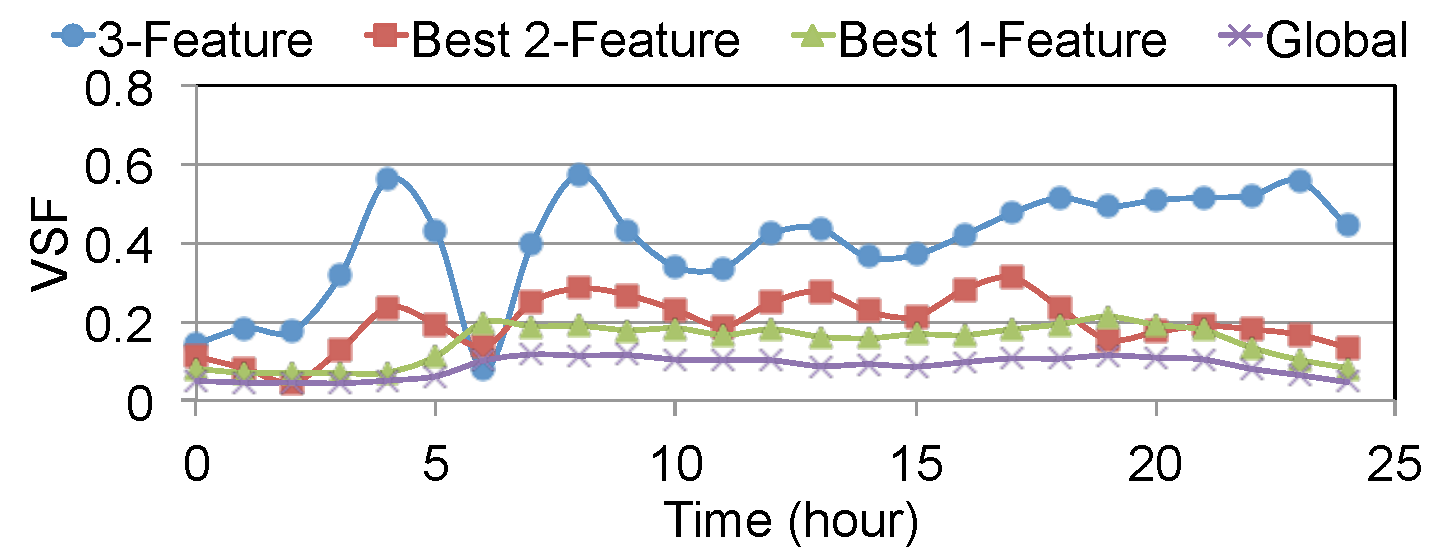
\includegraphics[width=0.65\textwidth]{figures/cfa-example-highdimension-timeseries.pdf}
\caption{The high VSF is only evident when three factors 
(CDN, ISP and geo-location) are combined.}
%\vspace{-0.2cm}
\label{fig:timeseries-expressive-model}
\end{figure}

 %One natural concern here is if this anecdotal evidence is an anomalous corner case.
% or if such high-dimensional 
%effects are  more pervasive. 
In practice, we find that such high-dimensional effects 
are the common case, rather than an anomalous corner case.  
For instance, more than 65\% of distinct
CDN-ISP-City values have VSF that is at least 50\% higher or 
lower than the VSF of sessions matching only one or 
two features (not shown). In other words, their quality is
affected by a combined effect of at least three features.

%\vyas{this doesnt address the concern. it  should have been across diff sessions/leaves :(}

\mypara{Limitation of existing solutions}
It might be tempting to develop  simple predictors; 
e.g., based on the last-hop 
connection by using average quality of history sessions 
with the same \fConnectionType value.
%\footnote{This is only an approximation to having the same last-hop capacity (we acknowledge that users of same connection type may have varying last-mile connection speed).}). 
However, they do not take into account the combined
impact of features on video quality.
Conventional machine learning techniques like Naive 
Bayes also suffer from the same limitation.
In Figures~\ref{subfig:quantitative-strawmen-lh} and 
\ref{subfig:quantitative-strawmen-nb},
we plot the actual JoinTime and the prediction
made by the last-hop predictor and Naive Bayes 
(from \texttt{Weka}~\cite{weka})
for 300 randomly sampled sessions.
The figures also show the mean relative error (
$\frac{|predicted-actual|}{actual}$).
For each session, the prediction algorithms train 
models using historical sessions within a 10-minute 
interval prior to the session under prediction.
It shows that the prediction error of both solutions is 
significant and two-sided (i.e., not fixable by
normalization).


\noindent{\bf Highly diverse structures of factors.}  
The factors that affect video quality vary across different sessions.
This means the prediction algorithm should be expressive enough
to predict quality for different sessions using 
different prediction models.
%\noindent\underline{Example of diversity:}
%Let us consider an illustrative example. 
%Many Flash video clients for whom Level3 
%edge servers provided high performance, and they had 
%good quality. 
%For these sessions, their quality is correlated with 
%a different set of features (\fCDN and \fPlayer) than 
%the example of high dimensionality (\fASN, \fCity and \fCDN).
For instance, the fact that many fiber-to-the-home (e.g., FiOS) 
users have high bitrates and people on 
 cellular connections have lower bitrates is largely due to 
the speed of their last-mile connection. In contrast, some video clients 
may experience video loading failures due to 
unavailability of specific content on some CDNs.
Chapter~\ref{ch:measurement}
has shown that many heterogeneous 
factors are correlated with video quality issues.
In Section~\ref{sec:cfa:outline}, we show  that 15\% of video 
sessions are impacted by more than 30 different combinations 
of features and give real examples of different factors that 
affect quality.

\noindent\underline{Limitation of existing solutions:}
To see why existing solutions are not sufficient, 
let us consider the $k$-nearest neighbor ($k$-NN) algorithm.
It does not handle diverse relationships between quality
and features, because the similarity between sessions
is based on the same function of features
independent of the specific session under prediction.
In Figure~\ref{subfig:quantitative-strawmen-nn},
we plot the actual values of JoinTime and the 
prediction made by $k$-NN with the same setup as 
Figure~\ref{subfig:quantitative-strawmen-lh}(b).
Similar to Naive Bayes and the last-hop predictor, 
$k$-NN has substantial prediction error.


\begin{figure}[t!]
\centering
\subfloat[Last hop (0.76)]
{
        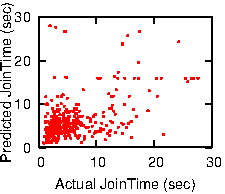
\includegraphics[width=0.3\textwidth]{figures/cfa-strawmen-scatter-comparison-naive.pdf}
        \label{subfig:quantitative-strawmen-lh}
}
\subfloat[Naive Bayes (0.61)]
{
        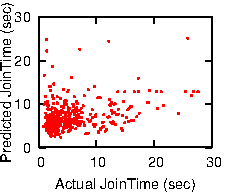
\includegraphics[width=0.3\textwidth]{figures/cfa-strawmen-scatter-comparison-2.pdf}
        \label{subfig:quantitative-strawmen-nb}
}
\subfloat[$k$-NN (0.63)]
{
        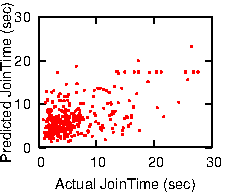
\includegraphics[width=0.3\textwidth]{figures/cfa-strawmen-scatter-comparison-1.pdf}
        \label{subfig:quantitative-strawmen-nn}
}
\caption{Prediction error of some existing solutions 
is substantial (mean of relative error in parentheses).}
%\vspace{-0.5cm}
\label{fig:quantitative-strawmen}
\end{figure}



\subsection{Challenge 2: Fresh Updates}
\label{subsec:fresh}

Video quality has significant temporal variability.
In Figure~\ref{fig:variability-all-metrics},
for each quality metric and combination of specific 
CDN, city and ASN, %(which reduces impact of the spatial variance), 
we compute the mean quality of sessions in each 
10-minute interval, and then plot the CDF of the 
relative standard deviation ($\frac{stddev}{mean}$)
%\footnote{Standard deviation divided by mean, which is used to normalize the scales of different quality metrics.} 
of the quality across different intervals.
In all four quality metrics of interest, we see 
significant temporal variability;
%on timescales of 10 minutes;
e.g., for 60\% of CDN-city-ASN combinations, 
the relative standard deviation of JoinTime across 
different 10-minute intervals is more than 30\%.
Such quality variability has also been confirmed in 
other studies (e.g.,~\cite{sigcomm12}).

The implication of such temporal variability
is that the prediction system must update models 
in near real-time.
In Figure~\ref{fig:strawman-staleness-all-metrics}, 
we use the same setup as 
Figure~\ref{fig:quantitative-strawmen}, except that the 
time window used to train prediction models is 
several minutes prior to the session under prediction.
The figure shows the impact of such staleness on 
the prediction error for JoinTime. 
For both algorithms, prediction error increases 
dramatically if the staleness exceeds 10 minutes. 
As we will see later, this negative impact of staleness 
on accuracy is not specific to these prediction 
algorithms (Section\ref{subsec:eval-scalability}). 
%This means the prediction system must update models  
%in near real-time.



\mypara{Limitation of existing solutions}
The requirement to use the most recent measurements
makes it infeasible to use computationally expensive models.
%models, such Support Vector Machines (SVM).
For instance, it takes at least one 
hour to train an SVM-based prediction model from 15K
quality measurements in a 10-minute interval for 
one video site, so the quality predictions 
will be based on information from more than one hour ago.


\begin{figure}[t!]
\centering
\subfloat[Temporal variability]
{
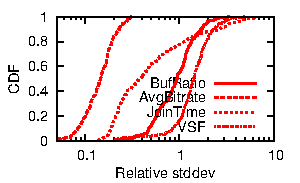
\includegraphics[width=.45\textwidth]{figures/cfa-stddev-metrics.pdf}
        \label{fig:variability-all-metrics}
}
\subfloat[Impact of staleness on accuracy]
{
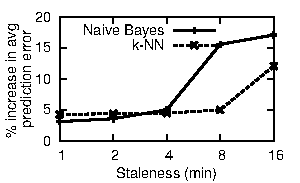
\includegraphics[width=.45\textwidth]{figures/cfa-strawman-staleness.pdf}
        \label{fig:strawman-staleness-all-metrics}
}
\caption{Due to significant temporal variability of video quality (left), 
prediction error increases dramatically with stale data (right).}
%\vspace{-0.2cm}
\label{fig:temporal-variability}
\end{figure}


%In summary, the ideal predictor should (a) capture the 
%complex relationship between features and video 
%quality, and (b) predict quality based on fresh data. 

%We will present \dda to achieve these goals in the
%next sections.

{
\begin{table}[h!]
%\begin{small}
\begin{tabular}{p{6cm}|p{3.5cm}|p{3cm}}
   &\textbf{Expressive models} & \textbf{Fresh updates} \\ \hline
Naive models (e.g., last-mile)                       & $\times$          & $\checkmark$         \\ \hline
Simple ML (e.g., NB, k-NN)                       & $\times$          & $\checkmark$         \\ \hline
Complex ML (e.g., SVM)	                            & ?                 & $\times$             \\ \hline 
{\bf The ideal (CFA)}                                 & {\bf $\checkmark$} & {\bf $\checkmark$}
\end{tabular}
%\end{small}
%\vspace{-0.3cm}
\caption{Analysis of existing solutions in the lense of the two challenges.}
%\vspace{-0.2cm}
\label{tab:qualitative-strawmen}
\end{table}
}












